\subsection{Parameterized shallow water equations}\label{sec:swe}
The final example considers reduced-order models of the shallow water equations with varying parameters. The governing system of PDEs for the shallow water equations is 
\begin{equation}\label{eq:swes}
\begin{split}
&\frac{\partial h}{\partial t} + \frac{\partial}{\partial \spatialvar }(  h u) + \frac{\partial}{\partial \spatialvarTwo }( h v) = 0\\
&\frac{\partial h u}{\partial t} + \frac{\partial}{\partial \spatialvar } (h u^2 + \frac{1}{2} \parameter_1 h^2) + \frac{\partial}{\partial \spatialvarTwo }( h u v) = 0\\
&\frac{\partial h v}{\partial t} + \frac{\partial}{\partial \spatialvar } (h u v) + \frac{\partial}{\partial \spatialvarTwo }( h v^2 +  \frac{1}{2} \parameter_1 h^2) = 0
\end{split}
\end{equation}
on the domain $(\spatialvar ,\spatialvarTwo ) \in \physDomain = [-5,5] \times [-5,5]$, $t \in [0,T]$
with $T=10$, and 
where $h,u,v: \physDomain \times [0,T] \rightarrow \RR{}$, with $h$ denoting the height
of the water surface, $u$ denoting the $\spatialvar$-velocity, and $v$
denoting the $\spatialvarTwo$-velocity.
The parameter $\parameter_1 \in \RR{+}$ is the ``gravity'' parameter.  In this example, we consider a set of parameterized initial conditions given by 
$$h(\spatialvar
,\spatialvarTwo ,0) = 1 + \parameter_2 e^{ -(\spatialvar  - 1)^2 -
(\spatialvarTwo  - 1)^2 }, \quad u(\spatialvar ,\spatialvarTwo ,0) =
v(\spatialvar ,\spatialvarTwo ,0) = 0,\quad (\spatialvar ,\spatialvarTwo ) \in
\physDomain,$$ which corresponds to a Gaussian pulse centered at $(1,1)$ with
a magnitude of $\parameter_2$. We consider a parameter domain
$(\parameter_1,\parameter_2)\in\parameterdomain = [3,9]\times [0.05,0.2]$.

\subsubsection{Description of FOM and generation of \spatialAcronym\ trial subspaces}
The full-order model again comprises a discontinuous Galerkin discretization of the system~\eqref{eq:swes}. We obtain the discretization 
by partitioning the domain into 128 elements of equal size in both the $\spatialvar$ and $\spatialvarTwo$ directions. Over each element, 
the solution is represented to second order via tensor product polynomials of order $p=1$. The resulting FOM dimension is $\fomdim = 196608$. The Rusanov flux is employed at the cell interfaces. Similarly to the previous section, spatial discretization via the discontinuous Galerkin method yields a dynamical system 
of the form
$$  \mass_{\text{DG}}\frac{d \state}{dt} = \velocity_{\text{DG}} (\state).$$
Time integration 
is again performed via the CN method with a time step of $\Delta t = 0.01$. The nonlinear system arising at each time step is solved via a Jacobian-free 
GMRES algorithm. We employ slip-wall boundary conditions at the edge of the domain. 


The reduced-order models again leverage POD to construct the \spatialAcronym\ trial basis with q-sampling based on snapshots of the FOM solution to select the sampling points. Once again, a uniform basis and sampling matrix is employed across all windows. The process used to construct the trial subspaces and weighting matrices for the ROMs is as follows:
\begin{enumerate}
\item Set the parameter-grid to be $\mathcal{D}_{\text{train}}  \{ 3,6,9 \} \times \{0.05,0.125,0.2\}$. 
\item Execute Algorithm~\ref{alg:pod_tlp} with inputs $N_{\text{skip}} = 2$, $\stateInterceptArg{} = \bz$, $\mathcal{D}_{\text{train}}$, $\romdim = \{ 83,143 ,223 \}$, and $\mathbf{T} = \mathbf{M}_{\text{DG}}$ to construct POD bases capturing $99.9999\%, \; 99.99999\%,$ and $99.999999\%$ of the energy, respectively.
\item Execute Algorithm~\ref{alg:qdeim_tlp} with inputs $\nskip = 2$, $\nsamples = 150$, $\mathcal{D}_{\text{train}}$ and $\mathbf{T} = \mathbf{M}_{\text{DG}}$ to construct a sample mesh of dimension $\mathbf{S} \in \{0,1\}^{1752\times \fomdim }$.
 \item Set $\stweightingMatOneArg{} = \mathbf{S} \mass_{\text{DG}}$. 
\end{enumerate}  
To depict the nature of the problem, Figure~\ref{fig:fom_sols_swe} presents surface plots for the surface height, $h$, at various time instances for the training parameter instance $\mu_1 = 9.0,\mu_2 = 0.125$.
\begin{figure}
\begin{center}
%\begin{subfigure}[t]{0.85\textwidth}
\begin{subfigure}[t]{0.49\textwidth}
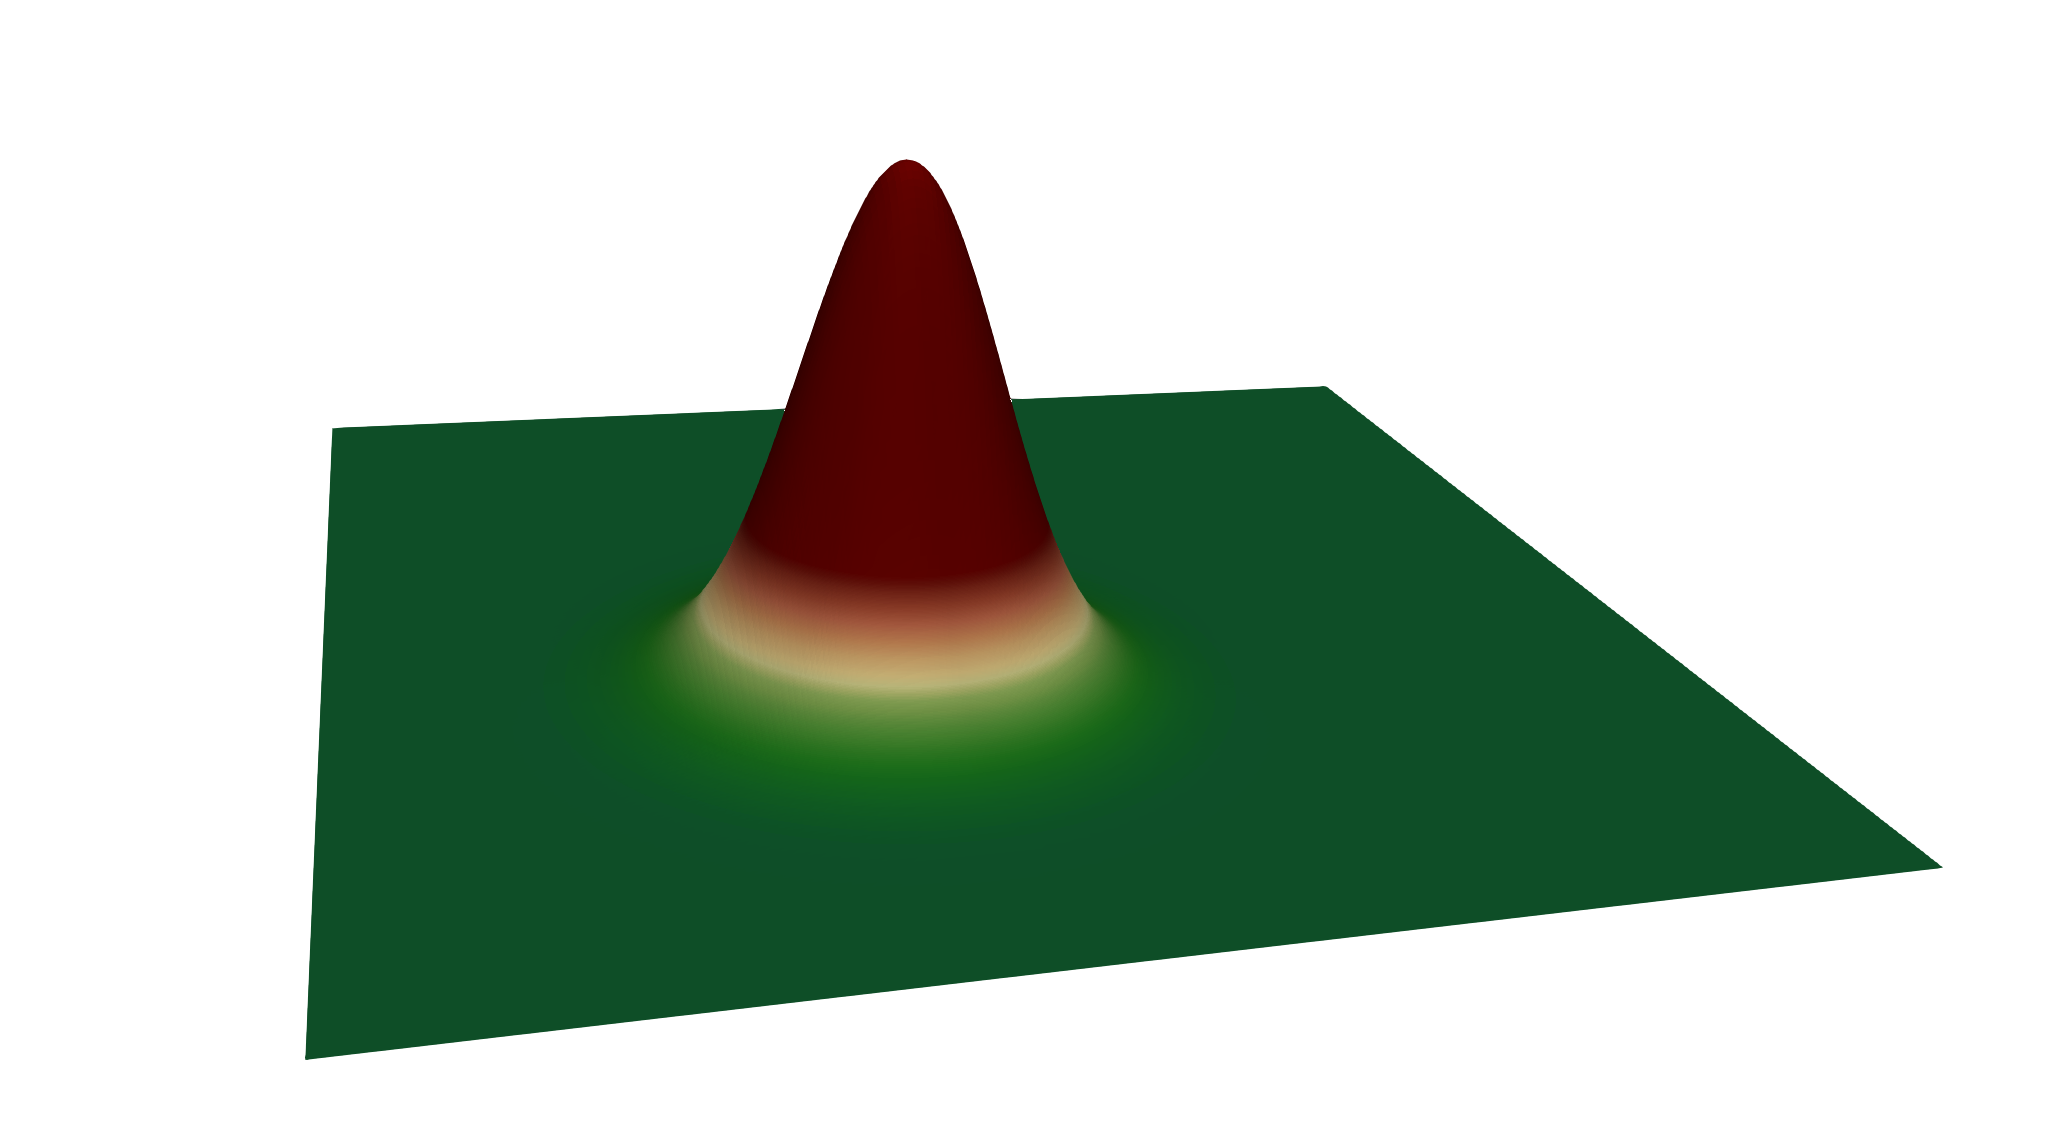
\includegraphics[trim={4cm 0cm 2cm 2cm},clip,width=1.0\linewidth]{figs/swe/h_t0.png}
\caption{$t=0.0$}
\end{subfigure}
\begin{subfigure}[t]{0.49\textwidth}
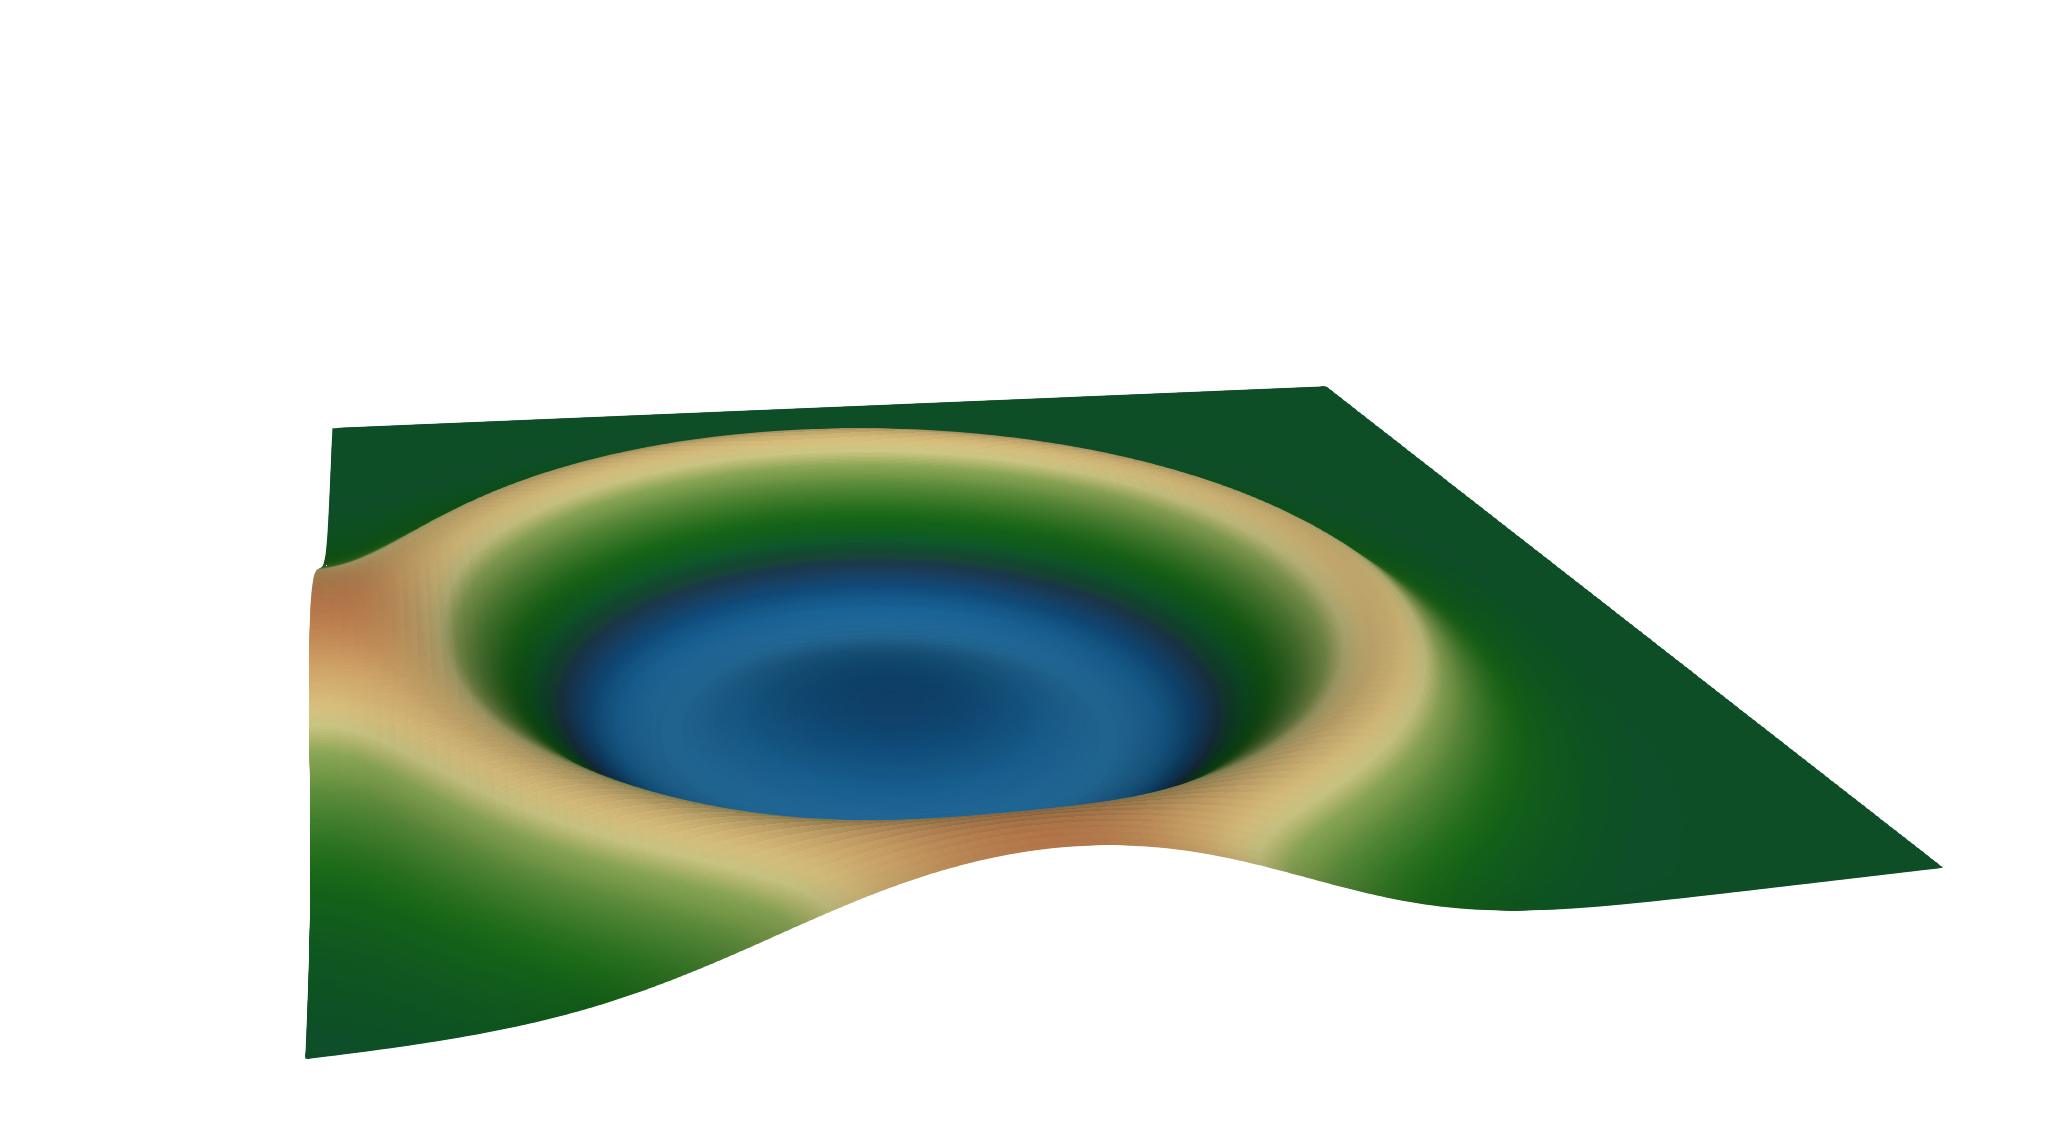
\includegraphics[trim={4cm 0cm 2cm 2cm},clip,width=1.0\linewidth]{figs/swe/h_t1.png}
\caption{$t=1.0$}
\end{subfigure}
%\begin{subfigure}[t]{0.85\textwidth}
\begin{subfigure}[t]{0.49\textwidth}
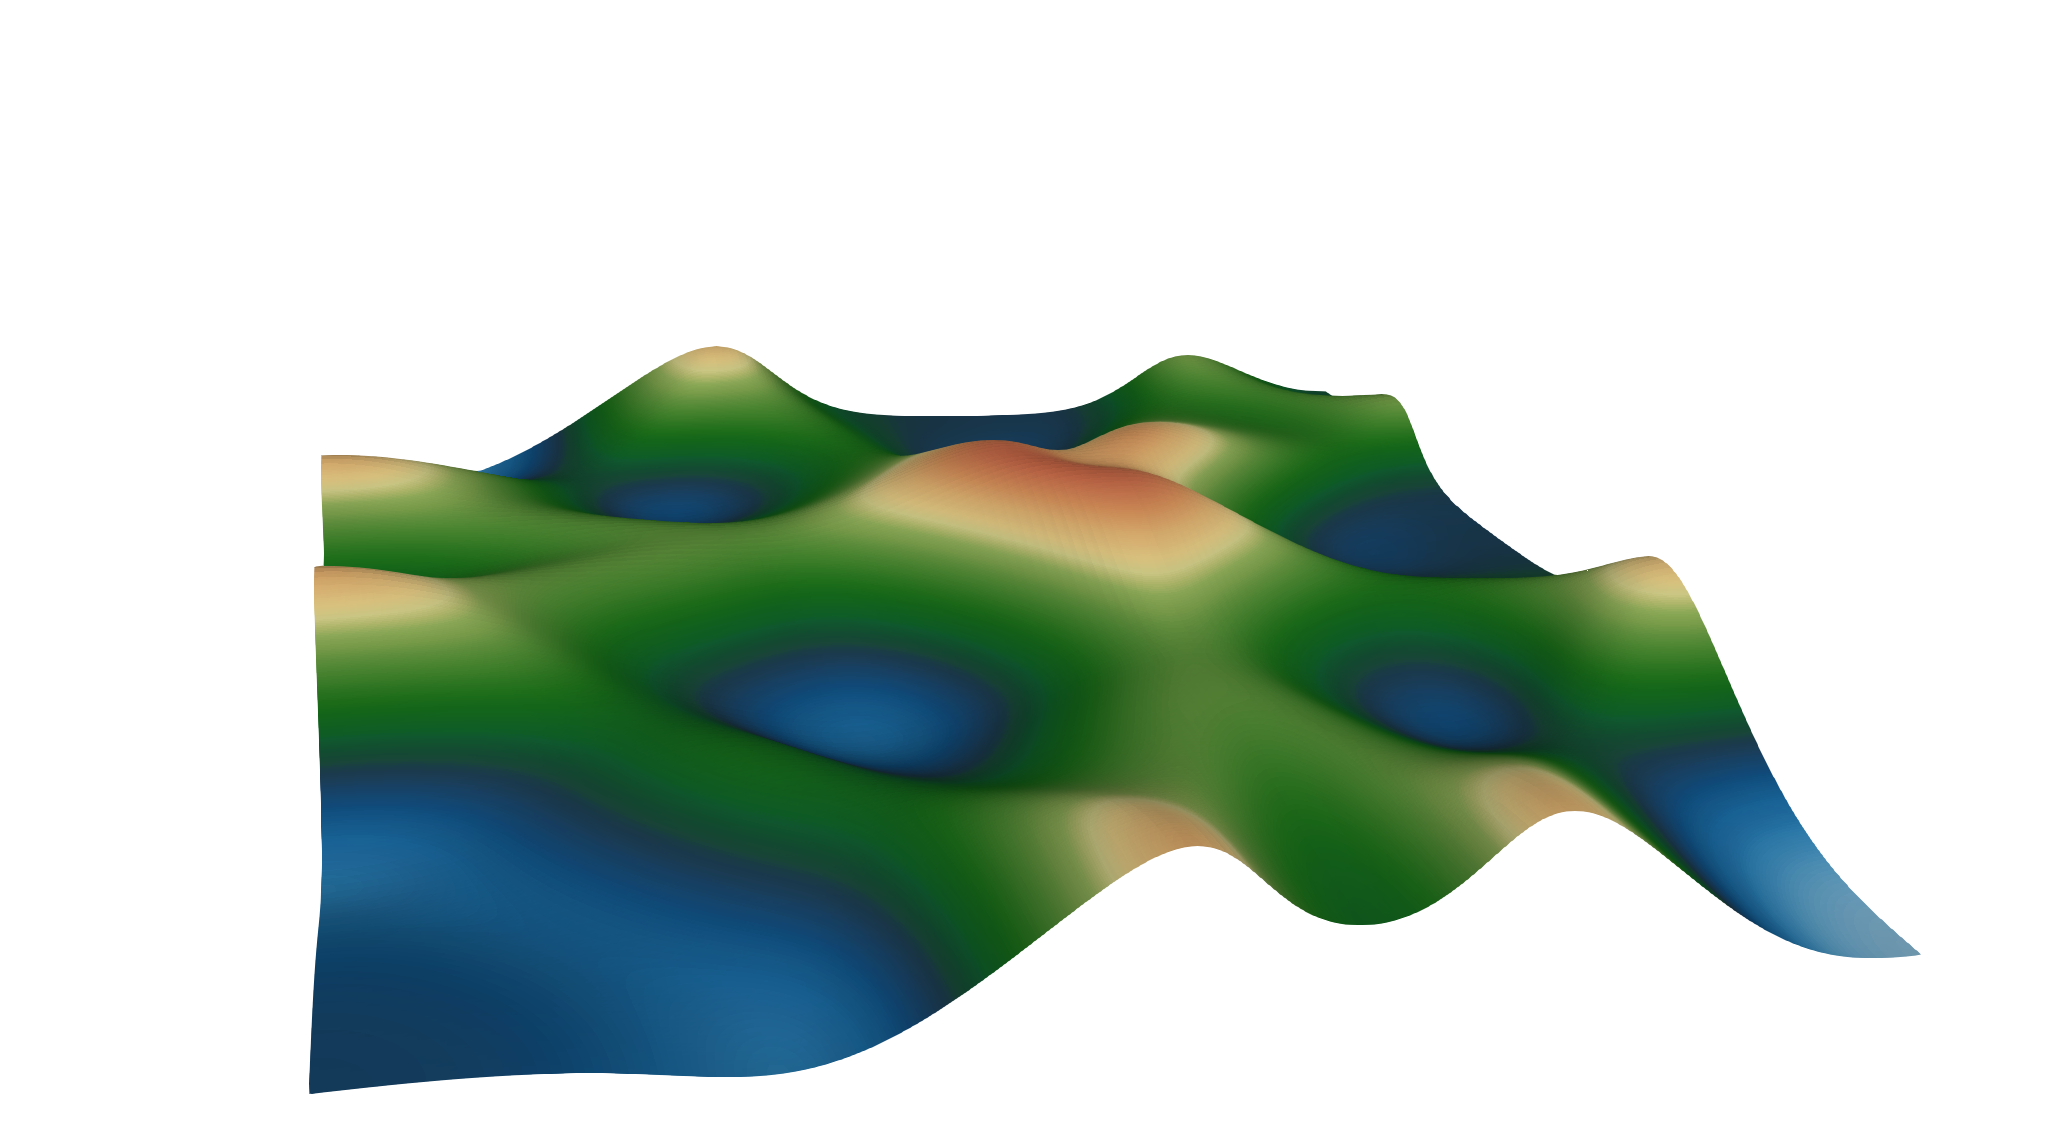
\includegraphics[trim={4cm 0cm 2cm 2cm},clip,width=1.0\linewidth]{figs/swe/h_t3.png}
\caption{$t=3.0$}
\end{subfigure}
\begin{subfigure}[t]{0.49\textwidth}
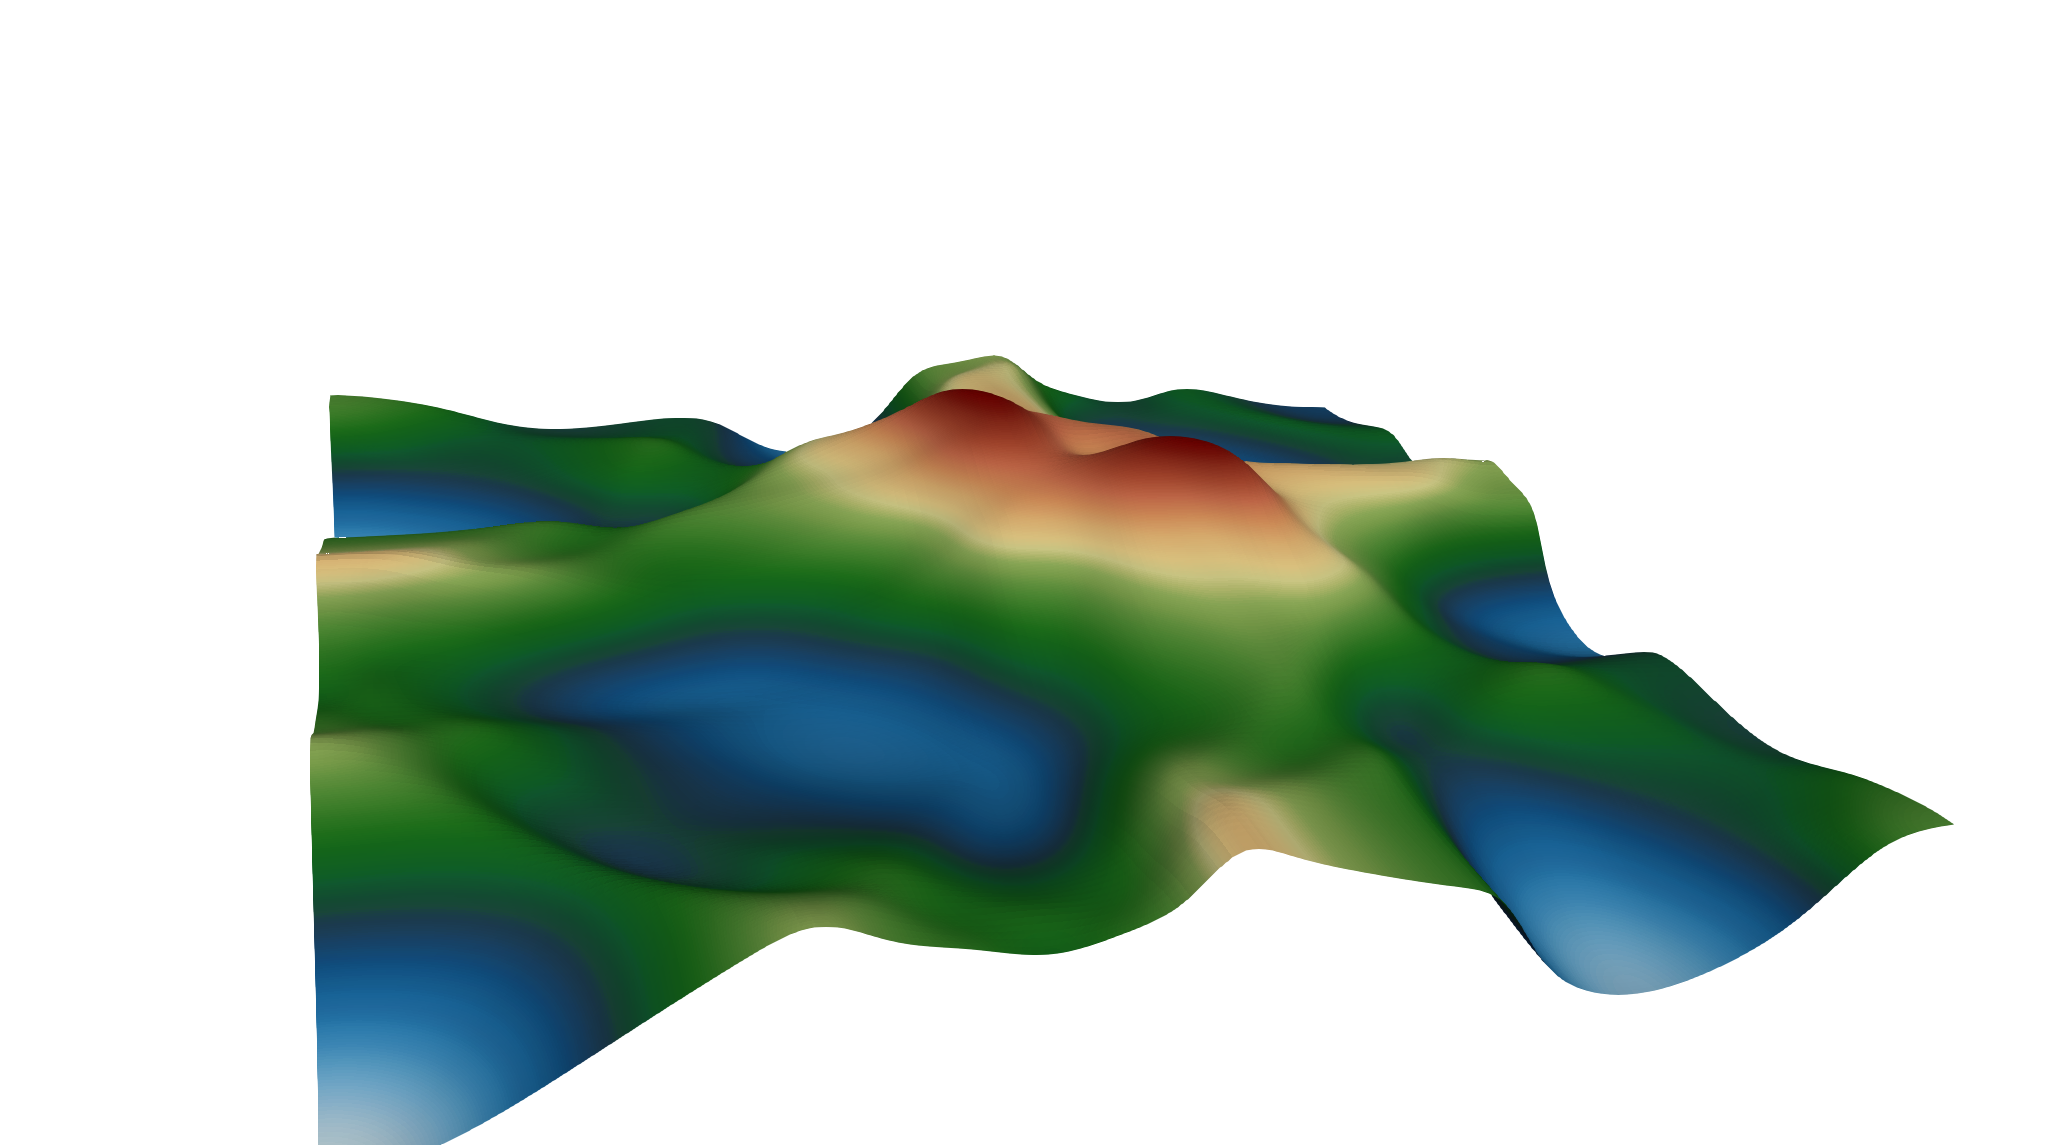
\includegraphics[trim={4cm 0cm 2cm 2cm},clip,width=1.0\linewidth]{figs/swe/h_t10.png}
\caption{$t=10.0$}
\end{subfigure}
\caption{Surface plots of the surface height, $h$, for the training parameter instance $\mu_1 = 9.0,\mu_2 = 0.125$.} 
\label{fig:fom_sols_swe}
\end{center}
\end{figure}


\subsubsection{Description of reduced-order models}\label{sec:swe_describe_roms}
We consider collocated ROMs based on the least-squares Petrov--Galerkin and \methodAcronym\ approaches. Details on the implementation of the methods is as follows:
\begin{itemize}

\item \textit{LSPG ROM with collocation}: We consider collocated LSPG ROMs, which are built on top of the FOM discretization using the CN scheme for temporal 
discretization. We employ a time step of $\Delta t  = 0.02$, which corresponds to the frequency at which snapshots were collected. 
The implementation is the same as previously described in Section~\ref{sec:sod_rom_description}, with the following exception: in the Gauss--Newton iteration used to solve the nonlinear least-squares problem arising at each time instance, a frozen Jacobian algorithm is employed, in where the Jacobian is updated every $n_{\text{update}}=10$ iterations. Appendix~\ref{appendix:gnupdate} details the impact of the update frequency of the Jacobian on the numerical results. The algorithm for the Gauss--Newton method with frozen Jacobians is presented in Algorithm~\ref{alg:colloc_gn_frozen} in Appendix~\ref{appendix:gnupdate}. We note here that the Gauss--Newton method with frozen Jacobians yields similar solutions to the standard Gauss--Newton approach, but at a much reduced computational cost.  
 
\item \textit{\methodAcronymROMs\ with collocation}: We consider \methodAcronymROMs\ solved via the direct method. The ROMs use the CN time discretization with a time step of 
$\Delta t = 0.02$. The implementation is the same as previously described in Section~\ref{sec:sod_rom_description}, with the exception that the ROMs employ the Gauss--Newton method with frozen Jacobians detailed above. 
%\begin{itemize}
%\item Direct Method: \methodAcronym ROMs solved via the direct method are again implemented with the same Crank--Nicolson time discretization with a nominal 
%time-step size of $\Delta t = 0.1$. 
%\end{itemize}
\end{itemize}
As an additional benchmark, we consider a time-local multivariate linear regression surrogate model. For each time instance, this surrogate operates by constructing a linear mapping from the input parameters, $(\mu_1 ,\mu_2)$, to the field solution at each grid point. Thus, the surrogate model is given as
\begin{equation}\label{eq:lin_surrogate}
\approxstateLR^n = {\approxstateLRIntercept}^n + \mu_1 \mathbf{c_1}^n + \mu_2 \mathbf{c_2}^n ,
\end{equation}
where $\approxstateLRIntercept^n \in \RR{\fomdim}$, $\mathbf{c_1}^n \in \RR{\fomdim}$, $\mathbf{c_2}^n \in \RR{\fomdim}$, $n=0,\ldots,N_t$, with $\fomdim = 196608$, are the model parameters. 
The surrogate model parameters are fits via \textsf{scikit-learn}~\cite{scikit-learn}. The same training data used for the ROM is used for the surrogate model.

\subsubsection{Numerical results at novel parameter instance}\label{sec:swe_results}
We investigate the performance of the reduced-order models at the novel parameter instance $(\mu_1, \mu_2) = (7.5,0.16)$. We emphasize that this parameter instance is not in the training set. We consider a set of WLS ROMs that minimize the residuals over $\DeltaSlabArg{n} \equiv \DeltaSlabArg{} = 0.04$, $0.1$, $0.2$, $0.5$, $1.0$, $2.0$, $5.0$, $10.0$, along with LSPG and the linear surrogate model~\eqref{eq:lin_surrogate}. First, Figure~\ref{fig:rom_sols_swe1} presents results for WLS ROMs at $\Delta T = 0.01,0.5,2.0,$ and $10.0$, as well as for the LSPG ROM and the linear regression surrogate model. Figure~\ref{fig:rom_sols_swe1h} depicts the evolution of the surface height at $(x,y) = (-2.4834,-2.4834)$ as a function of time, while Figure~\ref{fig:rom_sols_swe1e} depicts the relative $\elltwo$-error as a function of time. We first observe that the linear regression surrogate model performs significantly worse than all ROMs; this result demonstrates the complex dynamics of the problem. Next, we observe that LSPG yields poor solutions for later time instances. At $t=10$, LSPG only yields a marginally better prediction than the linear surrogate model. We next observe the WLS ROMs to yield improved solutions as compared to LSPG. We observe that the evolution of the surface height as a function of time is better characterized; specifically we once again observe that growing the window size yields smoother solutions. Next, Figure~\ref{fig:rom_hsols_swe} presents surface plots of the surface height, $h$, for the FOM and various ROMs at $t = 10.0$. We observe the LSPG solution to be contaminated by spurious oscillations and, as a result, it fails to accurately characterize the FOM. On the other hand, we observe the WLS ROMs to yield smooth solutions that accurately characterize the FOM.
 


\begin{figure}
\begin{center}
\begin{subfigure}[t]{0.49\textwidth}
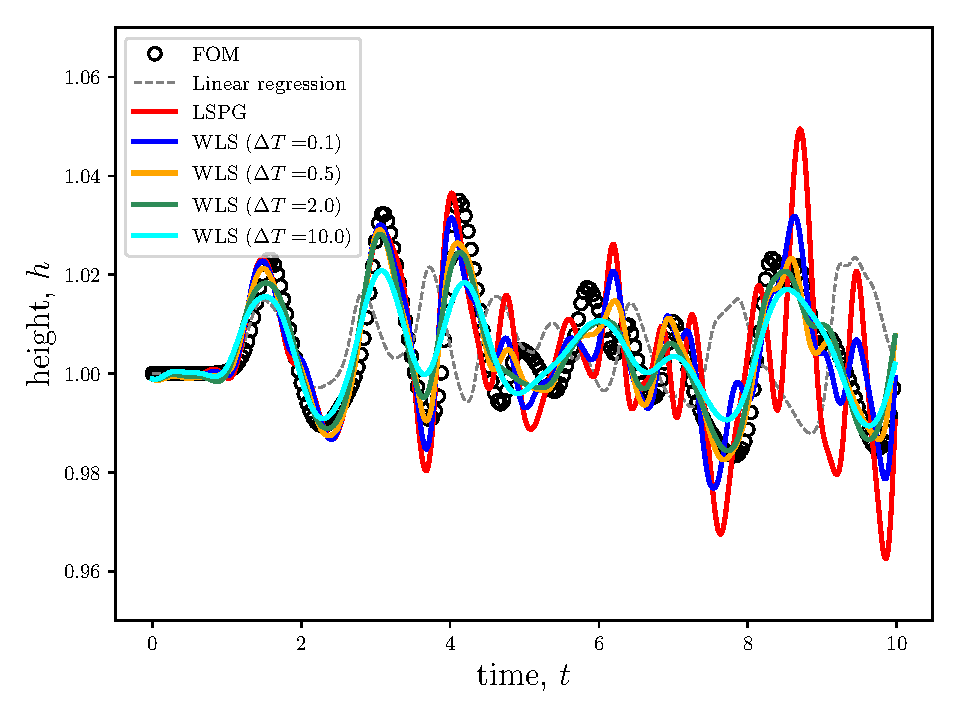
\includegraphics[trim={0cm 0cm 0cm 0cm},clip,width=1.0\linewidth]{figs/swe/swe_h_vs_t_K83.pdf}
\caption{Surface height.}
\label{fig:rom_sols_swe1h}
\end{subfigure}
\begin{subfigure}[t]{0.49\textwidth}
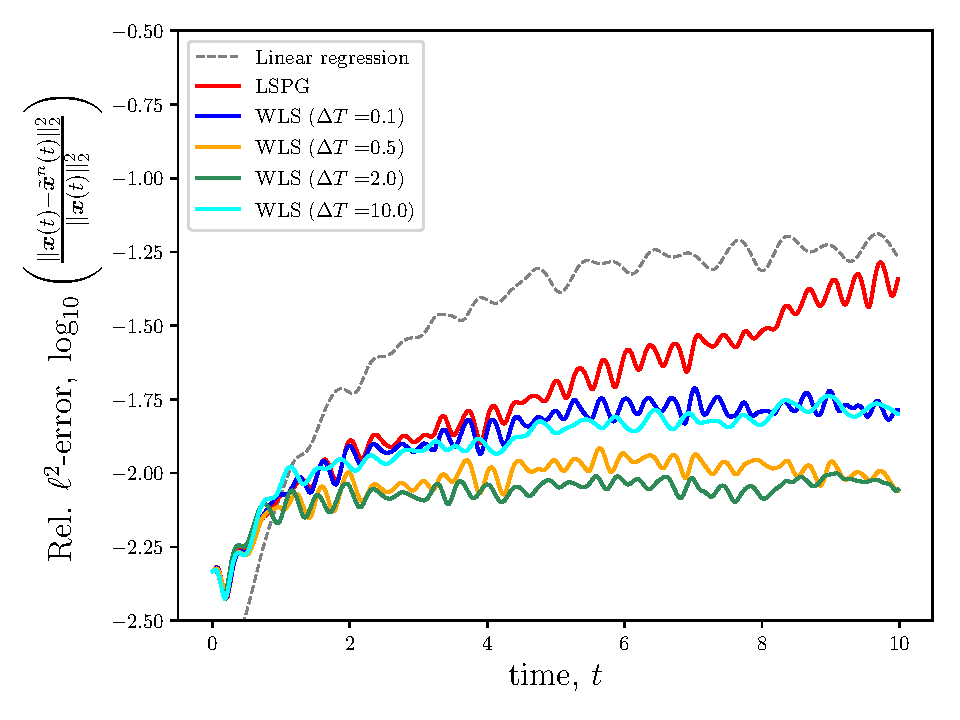
\includegraphics[trim={0cm 0cm 0cm 0cm},clip,width=1.0\linewidth]{figs/swe/swe_error_vs_t_K83.pdf}
\caption{Relative error.}
\label{fig:rom_sols_swe1e}
\end{subfigure}
\caption{Surface height at $(x,y) = (-2.4834,-2.4834)$ (left) and relative error (right) as a function of time.} 
\label{fig:rom_sols_swe1}
\end{center}
\end{figure}

\begin{figure}
\begin{center}
%\begin{subfigure}[t]{0.85\textwidth}
\begin{subfigure}[t]{0.49\textwidth}
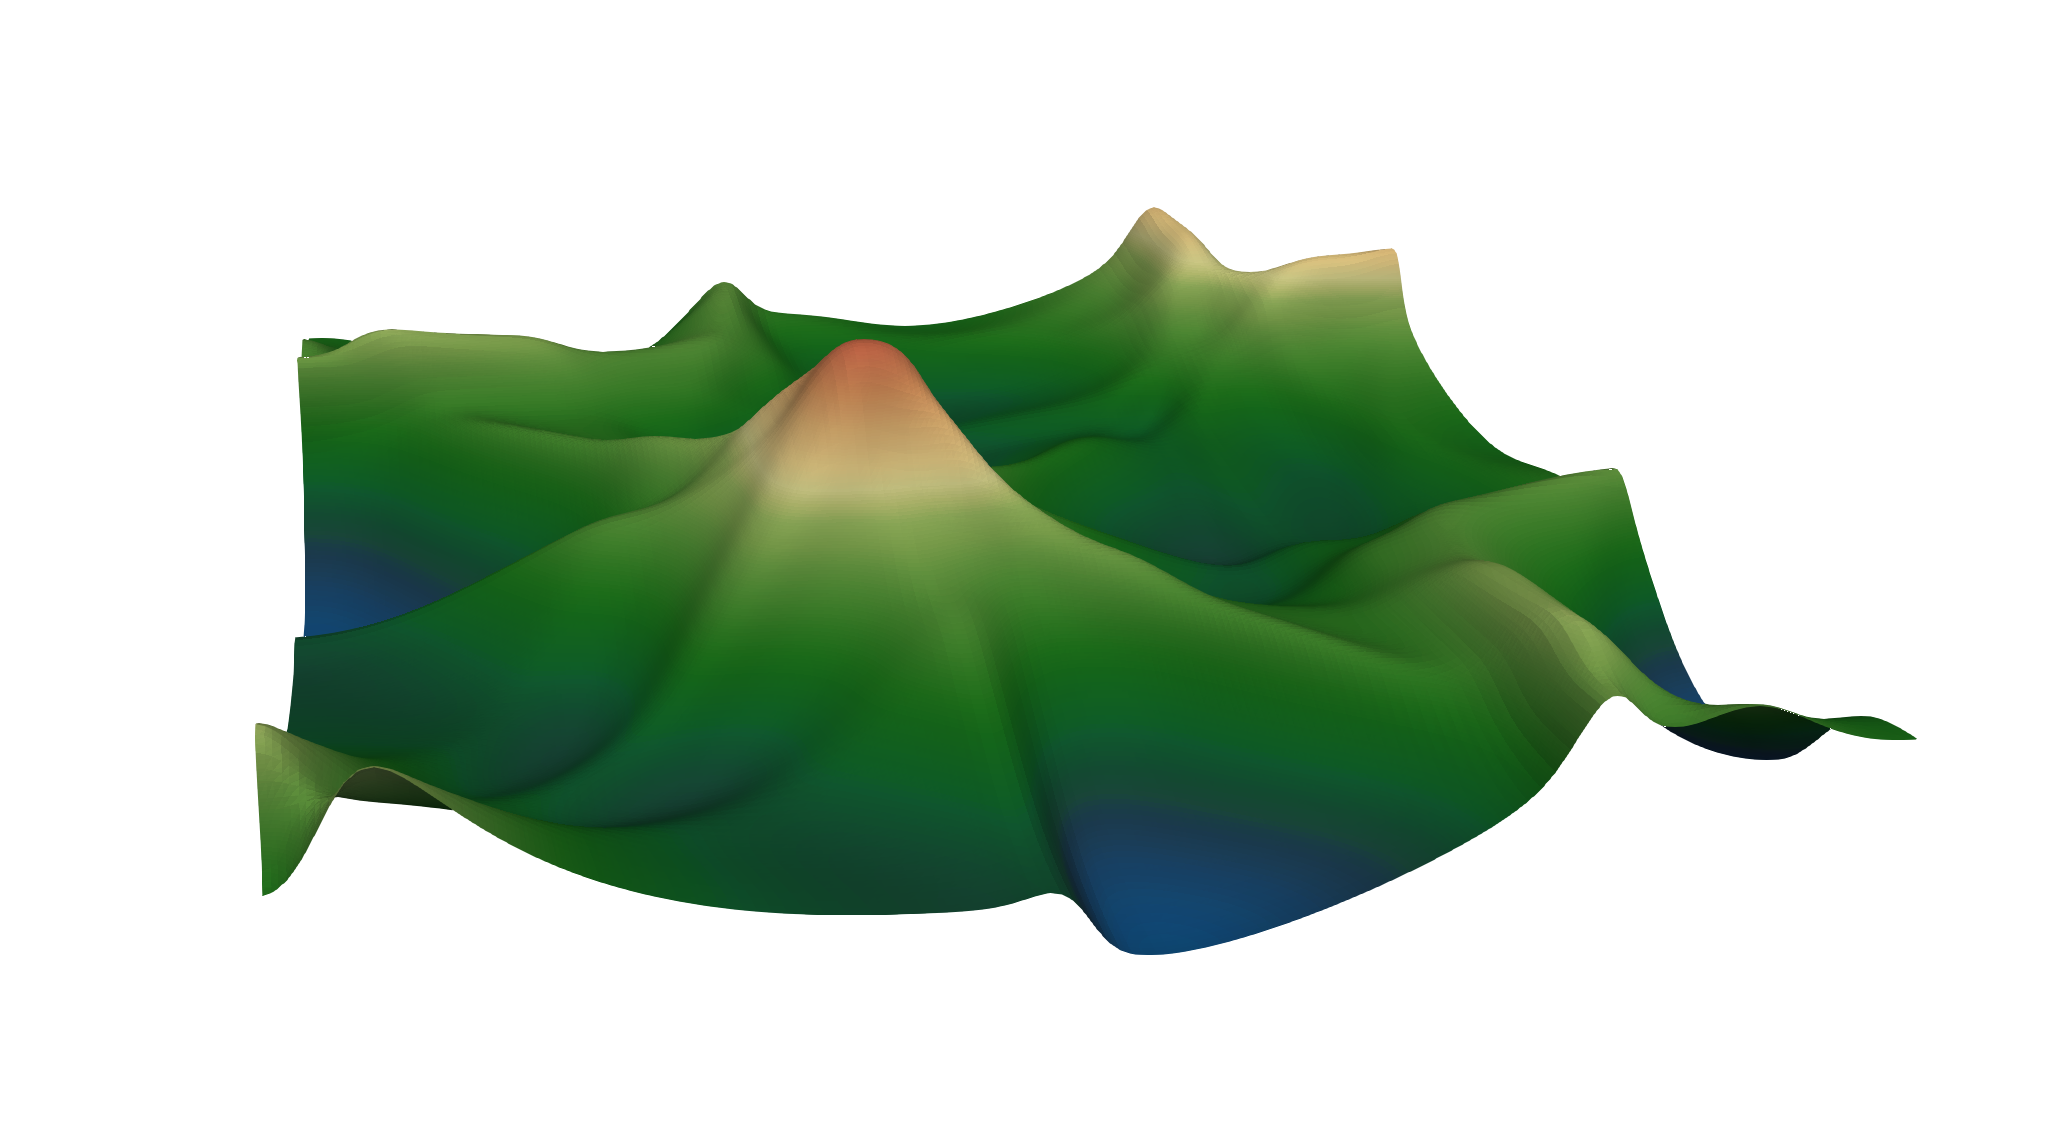
\includegraphics[trim={4cm 0cm 2cm 2cm},clip,width=1.0\linewidth]{figs/swe/h_fom_t50.png}
\caption{FOM}
\end{subfigure}
\begin{subfigure}[t]{0.49\textwidth}
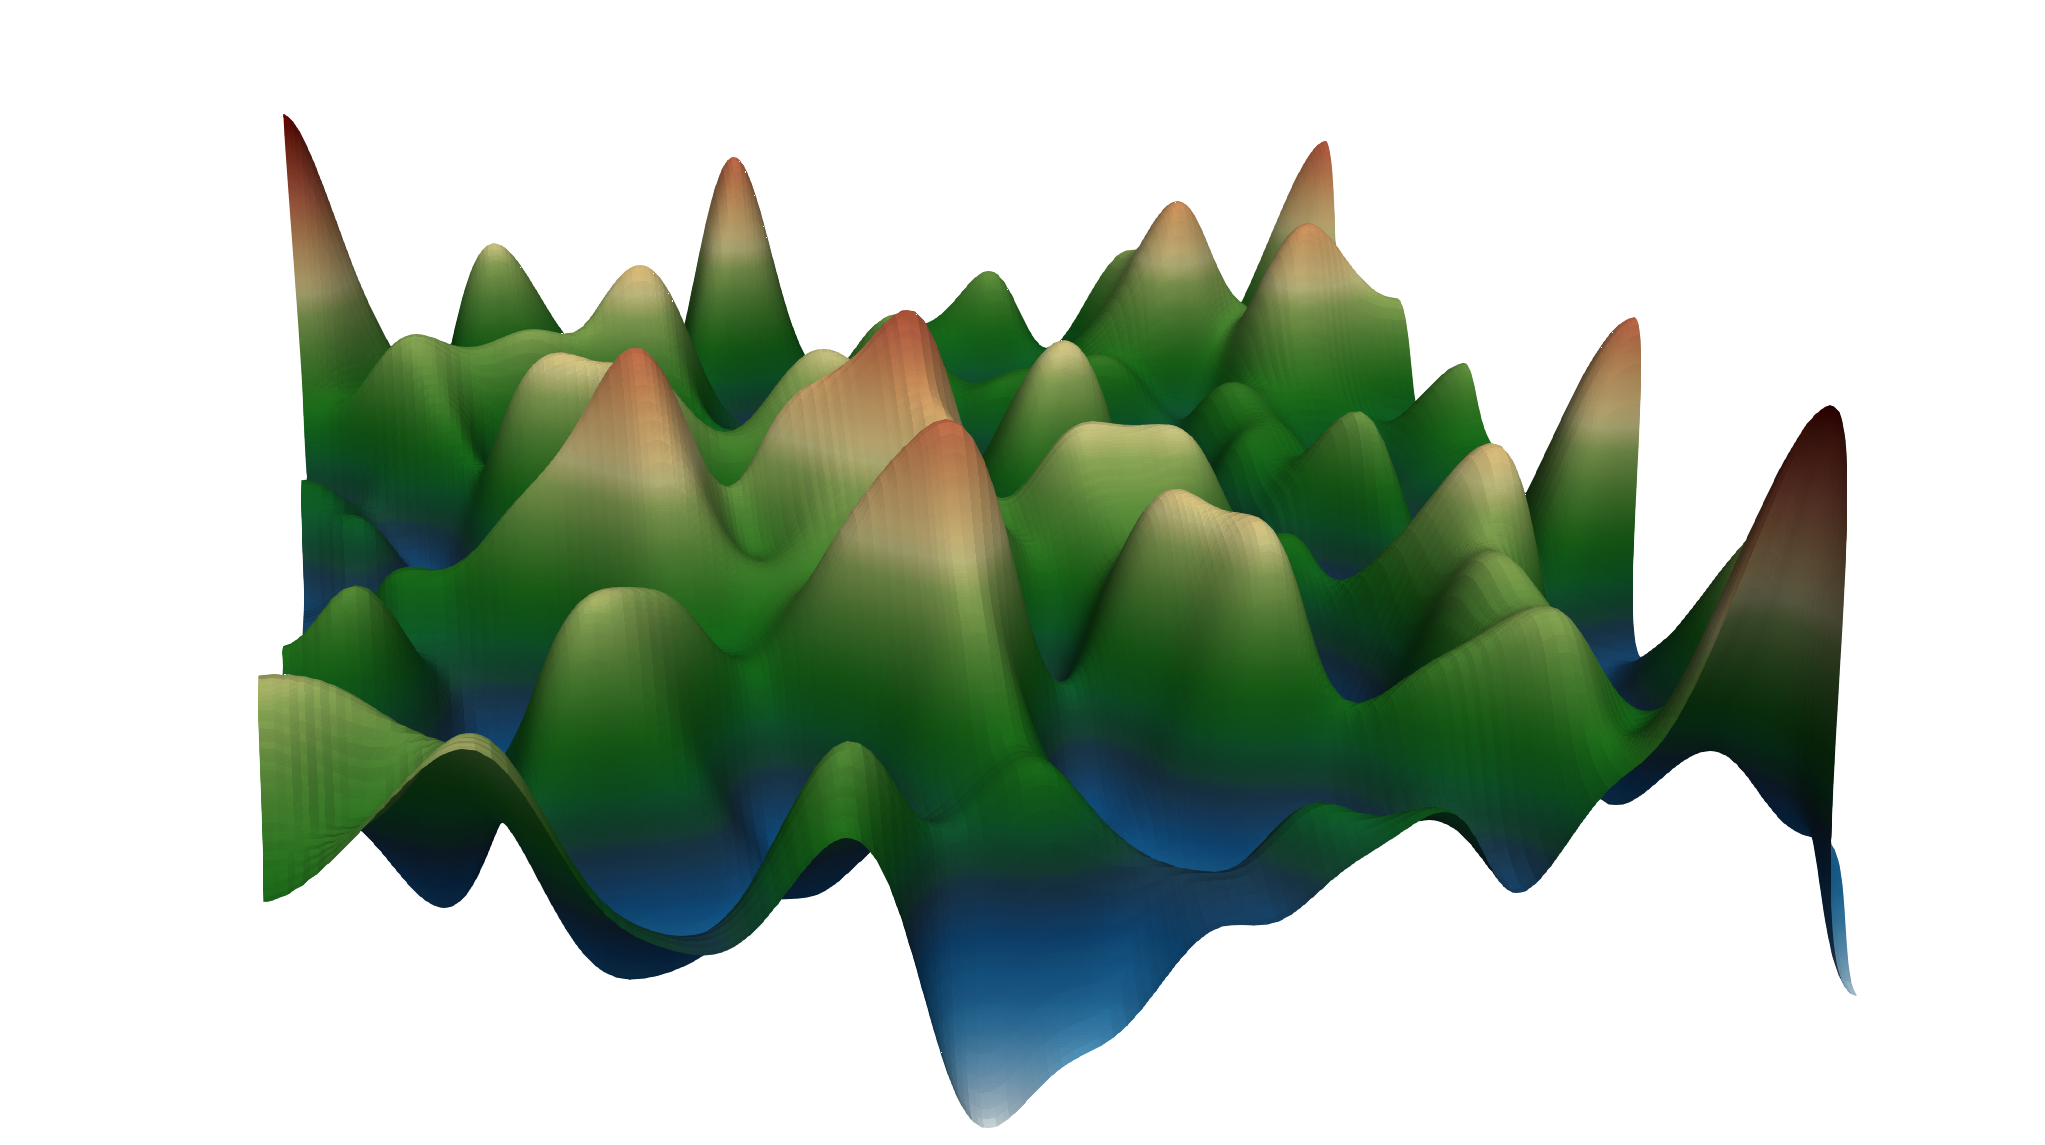
\includegraphics[trim={4cm 0cm 2cm 2cm},clip,width=1.0\linewidth]{figs/swe/h_lspg_t50.png}
\caption{LSPG}
\end{subfigure}
%\begin{subfigure}[t]{0.85\textwidth}
\begin{subfigure}[t]{0.49\textwidth}
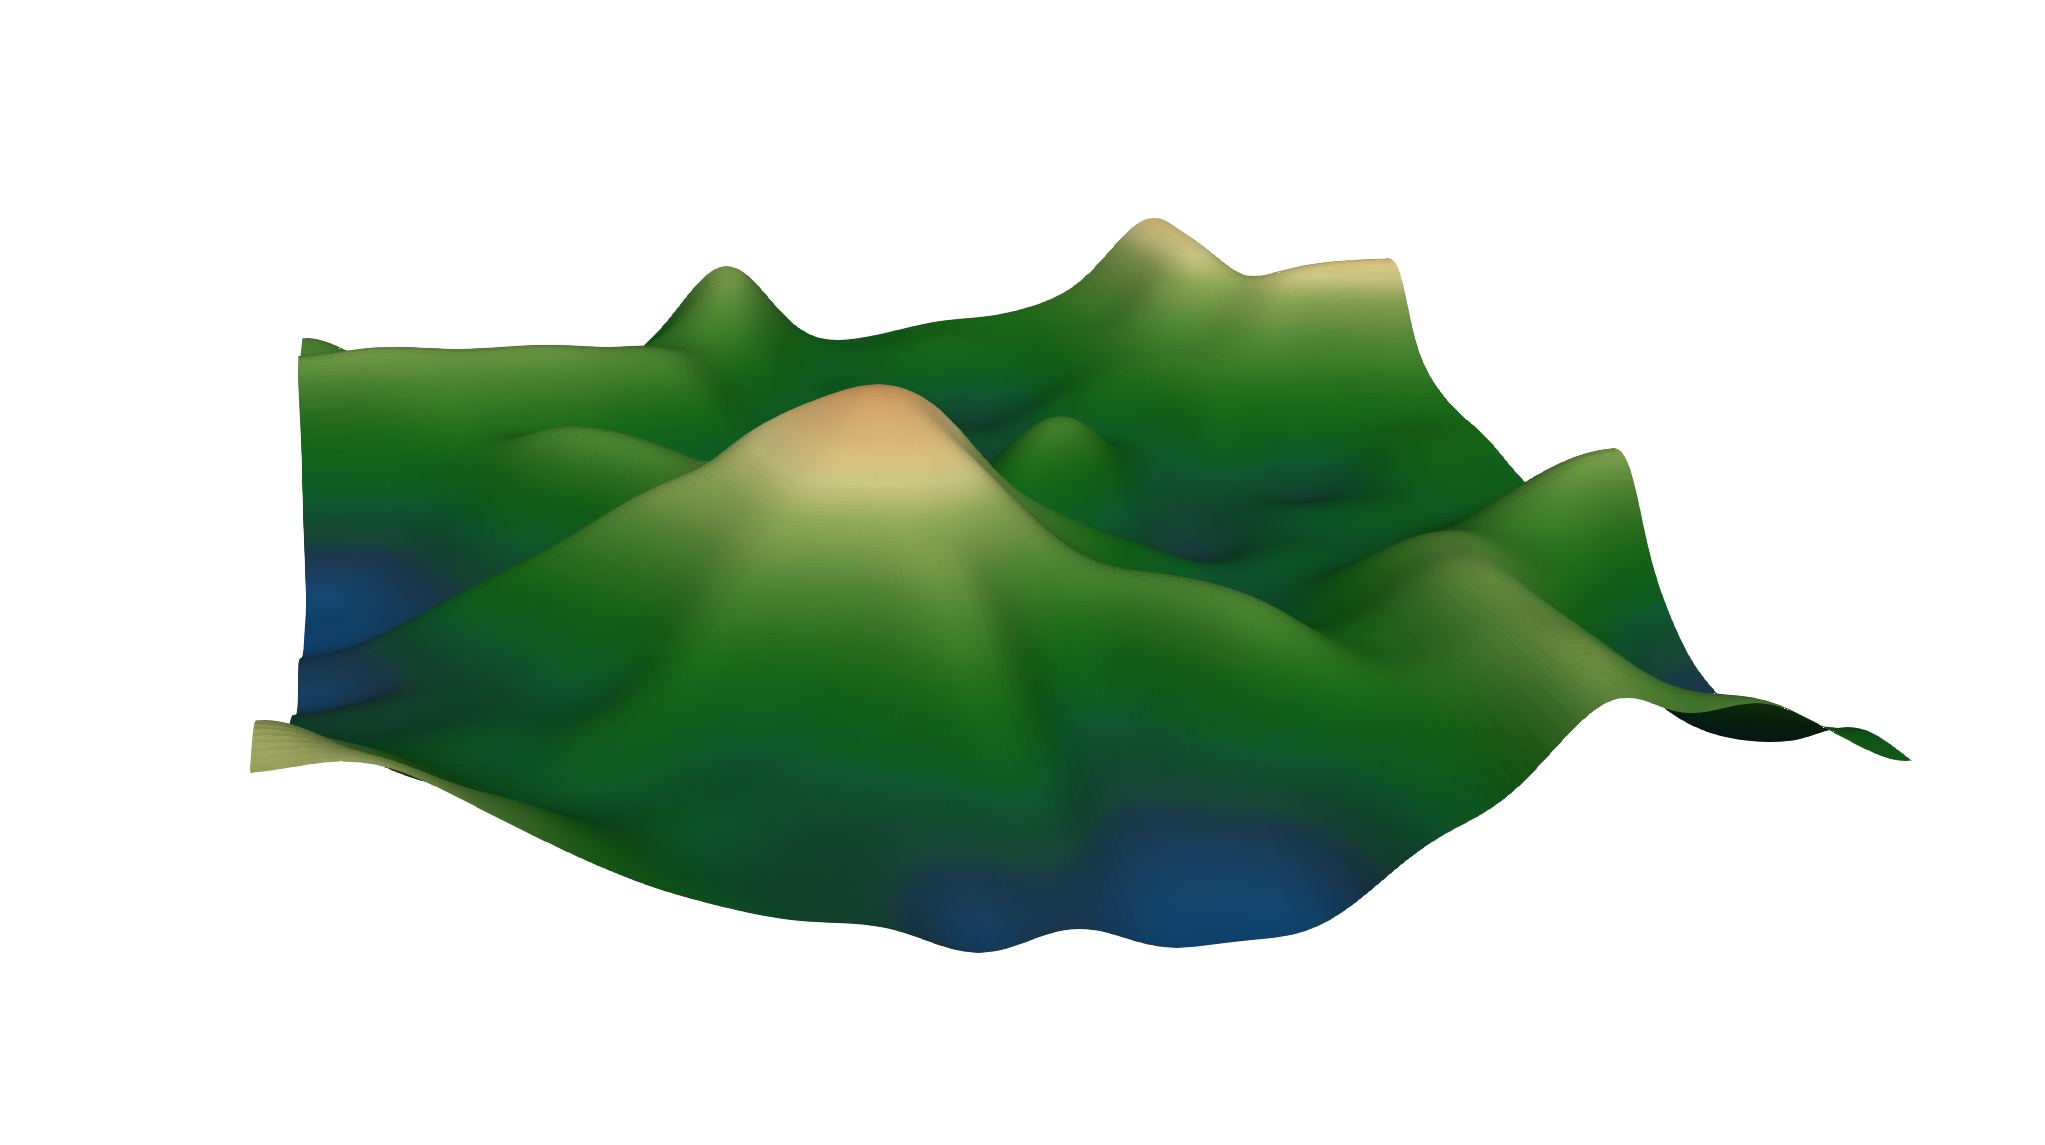
\includegraphics[trim={4cm 0cm 2cm 2cm},clip,width=1.0\linewidth]{figs/swe/h_wls_DT05_t50.png}
\caption{WLS ($\Delta T = 0.5$)}
\end{subfigure}
\begin{subfigure}[t]{0.49\textwidth}
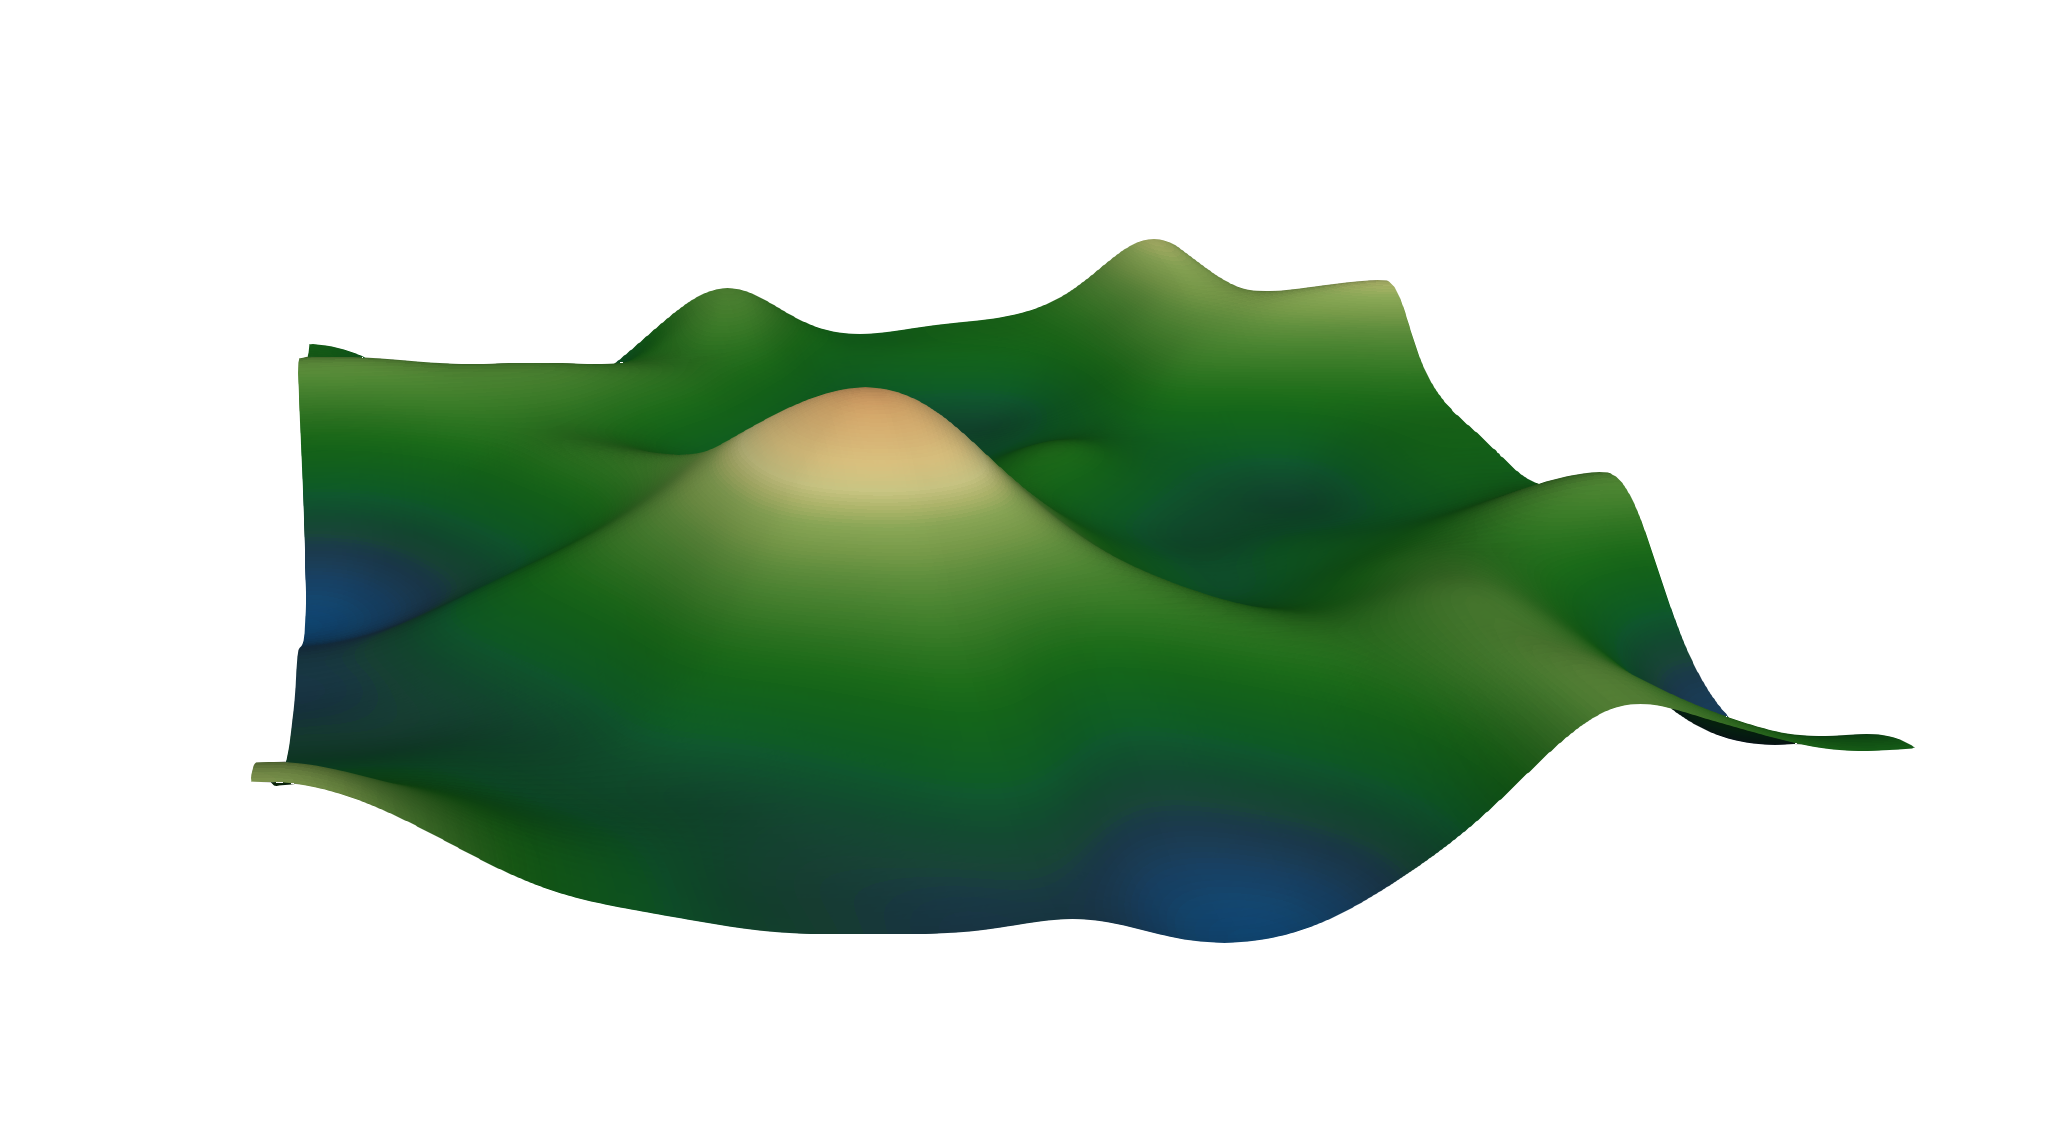
\includegraphics[trim={4cm 0cm 2cm 2cm},clip,width=1.0\linewidth]{figs/swe/h_wls_DT20_t50.png}
\caption{WLS ($\Delta T=2.0$)}
\end{subfigure}
\caption{Surface plots of the surface height, $h$, at $t=10.0$ for the novel parameter instance $\mu_1 = 7.5,\mu_2 = 0.16$ as predicted by the FOM and various ROMs.} 
\label{fig:rom_hsols_swe}
\end{center}
\end{figure}

Figure~\ref{fig:rom_swe_metrics} depicts the impact of the window size on the relative error and residual norms. The time-integrated $\elltwo$-error of the linear surrogate model is additionally shown for reference. We make the same observations as before: increasing the window size leads to a monotonic decrease in the time-integrated residual norm, but not in the time-integrated error norm. We observe that the time integrated $\elltwo$-error is lowest for an intermediate window size. At $\Delta T = 1$, the time-integrated $\elltwo$-error of the WLS ROM is approximately half that of LSPG. We additionally note that all ROMs are significantly more accurate than the linear surrogate model. Similarly, WLS with $\Delta T = 10.0$ yields a time-integrated residual norm that is almost three orders of magnitude lower than LSPG. 


\begin{figure}
\begin{center}
%\begin{subfigure}[t]{0.85\textwidth}
\begin{subfigure}[t]{0.49\textwidth}
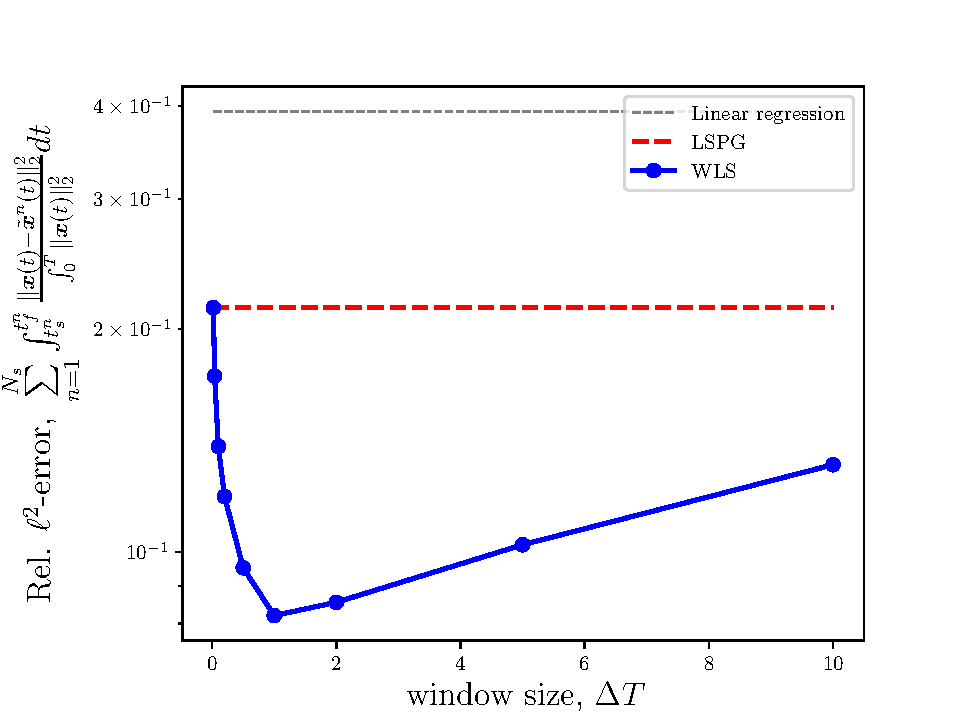
\includegraphics[trim={0cm 0cm 0cm 0cm},clip,width=1.0\linewidth]{figs/swe/swe_windowSize_vs_error_K83.pdf}
\caption{Relative time-integrated $\elltwo$-error.}
\end{subfigure}
\begin{subfigure}[t]{0.49\textwidth}
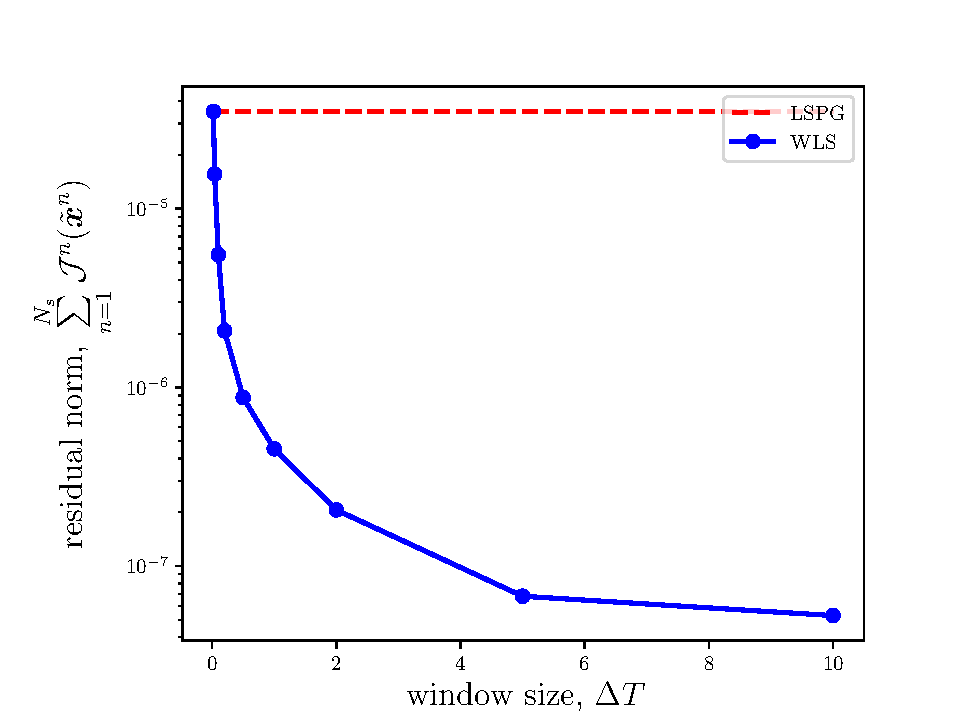
\includegraphics[trim={0cm 0cm 0cm 0cm},clip,width=1.0\linewidth]{figs/swe/swe_windowSize_vs_residual_K83.pdf}
\caption{Time-integrated residual norm.}
\end{subfigure}
%\begin{subfigure}[t]{0.85\textwidth}
\caption{Time-integrated error metrics of the LSPG and WLS ROMs as a function of window size} 
\label{fig:rom_swe_metrics}
\end{center}
\end{figure}

Figure~\ref{fig:rom_swe_timings} presents timings for the various ROMs as a function of the window size. We note that, as described in Section~\ref{sec:swe_describe_roms}, all ROMs employ a Gauss--Newton solve with a Jacobian update frequency of $n_{\text{update}} = 10$; the sensitity of the results to this parameter are detailed in Appendix~\ref{appendix:gnupdate}. We again observe that the cost of WLS grows with window size: WLS with $\Delta T = 10.0$ ($=500\Delta t$) incurs a 5x increase in computational cost with respect to LSPG. With respect to the FOM, we observe LSPG to result in a $20$x speedup, while WLS with the largest window size $\Delta T = 10.0$ yields a $4$x speedup.  
\begin{figure}
\begin{center}
%\begin{subfigure}[t]{0.85\textwidth}
\begin{subfigure}[t]{0.49\textwidth}
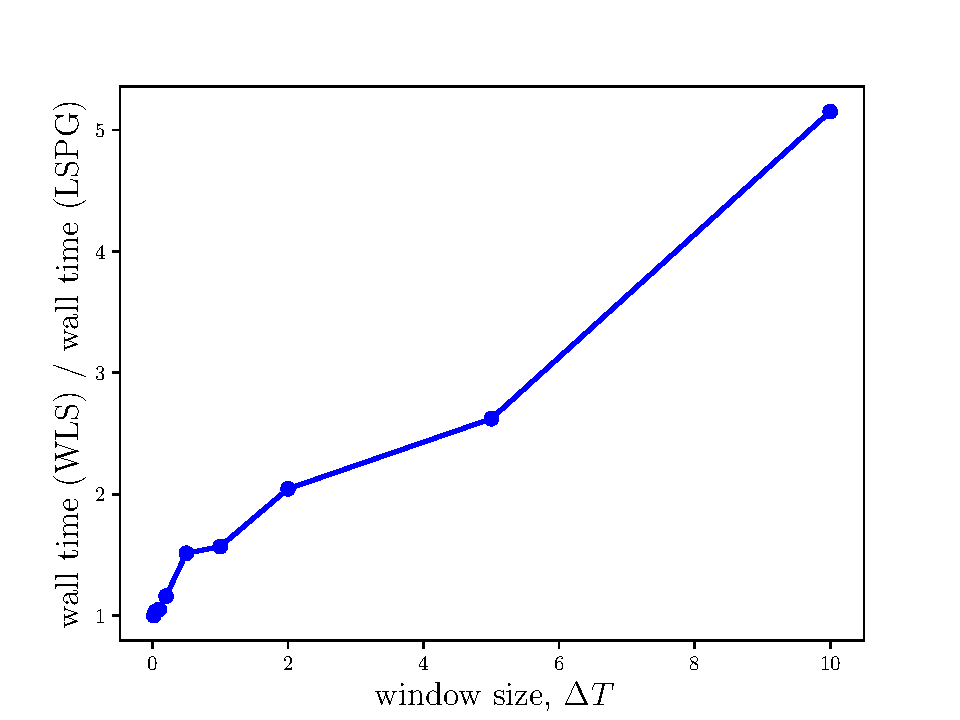
\includegraphics[trim={0cm 0cm 0cm 0cm},clip,width=1.0\linewidth]{figs/swe/swe_windowSize_vs_walltimeLspg_updateFreq_K83.pdf}
\end{subfigure}
\begin{subfigure}[t]{0.49\textwidth}
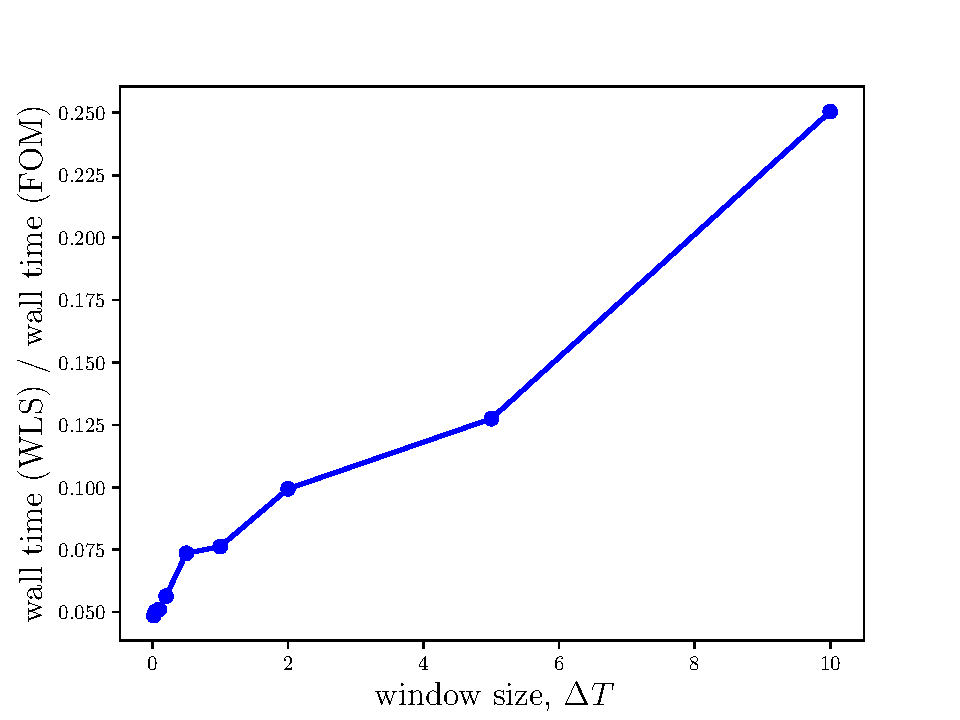
\includegraphics[trim={0cm 0cm 0cm 0cm},clip,width=1.0\linewidth]{figs/swe/swe_windowSize_vs_walltimeFom_updateFreq_K83.pdf}
\end{subfigure}
%\begin{subfigure}[t]{0.85\textwidth}
\caption{Wall clock times as a function of window size relative to LSPG (left) and the FOM (right).} 
\label{fig:rom_swe_timings}
\end{center}
\end{figure}

We next assess the impact of the basis dimension on the results. Figure~\ref{fig:rom_swe_converge} summarizes the performance of WLS and LSPG ROMs as a function of basis dimension. We first observe that LSPG, and WLS with smaller window sizes, do not display monotonic convergence with increasing basis dimension. 
We expect that this lack of convergence is due to the fact that, as the basis dimension increases, the ROM trial space can represent sharper gradients. Without proper stabilization, this can yield spurious oscillations, as previously observed in Figure~\ref{fig:rom_hsols_swe}. As the window size increases, the ROM is more stable and, thus, increasing the basis dimension yields improved solutions. 
For window sizes of $\Delta T \ge 0.5$, we observe that increasing the basis dimension leads to a monotonic decrease in both the time-integrated $\elltwo$-error and residual norm. 

\begin{figure}
\begin{center}
%\begin{subfigure}[t]{0.85\textwidth}
\begin{subfigure}[t]{0.49\textwidth}
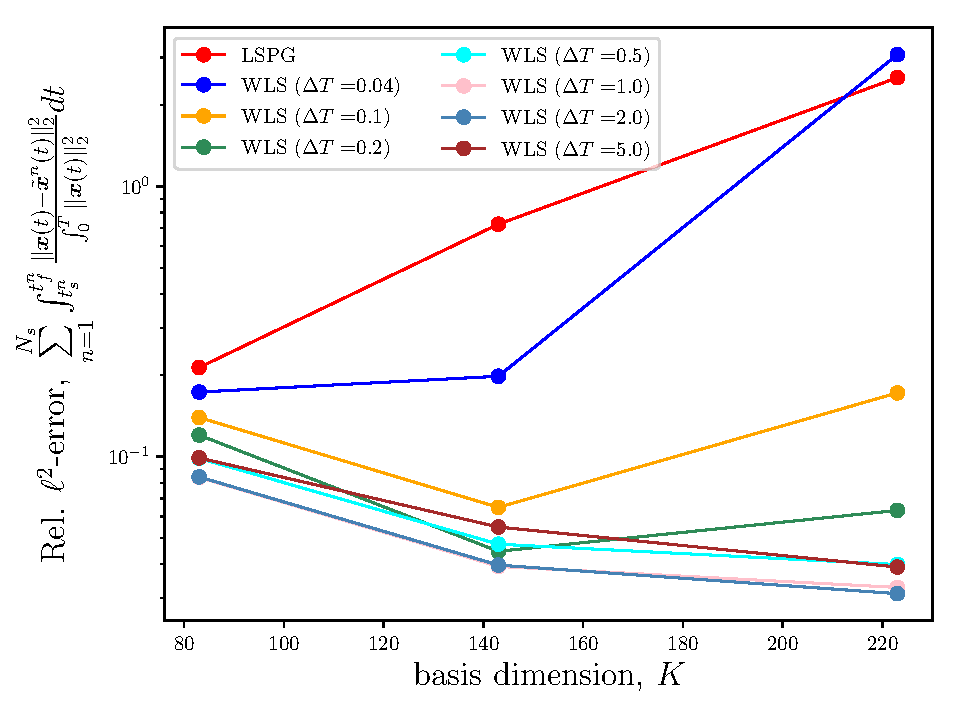
\includegraphics[trim={0cm 0cm 0cm 0cm},clip,width=1.0\linewidth]{figs/swe/swe_converge_error.pdf}
\caption{Relative time-inegrated $\elltwo$-error.}
\end{subfigure}
\begin{subfigure}[t]{0.49\textwidth}
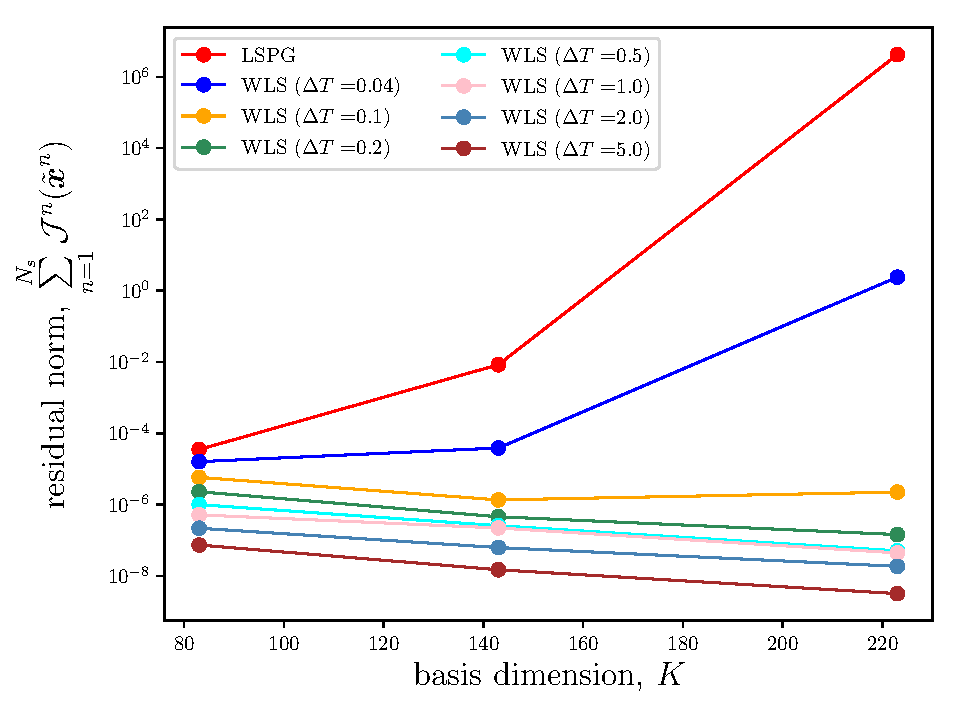
\includegraphics[trim={0cm 0cm 0cm 0cm},clip,width=1.0\linewidth]{figs/swe/swe_converge_resid.pdf}
\caption{Time integrated residual norm.}
\end{subfigure}
%\begin{subfigure}[t]{0.85\textwidth}
\caption{Time-integrated error metrics of the LSPG and WLS ROMs as a function of basis dimension.} 
\label{fig:rom_swe_converge}
\end{center}
\end{figure}

Lastly, Figure~\ref{fig:rom_swe_pareto} presents Pareto plots for the time-integrated $\elltwo$-error and residual as a function of wall-clock times for ROMs with basis dimensions $K = 83,143,223$ and window sizes $\Delta T = 0.04, 0.1,0.2,0.5,1.0,2.0,$ and $5.0$, along with LSPG. We again observe ROMs employing an intermediate window size to be Pareto-optimal for the time-integrated $\elltwo$-error. It is interesting to note that the error vs. wall time curves for WLS ($\Delta T = 0.01$, $0.02$, $0.05$, $1.0$ ,$2.0$) fall almost on top of each other. Lastly, we observe that larger window sizes with lower basis dimensions are Pareto optimal for the residual. For instance, we observe that WLS with $\Delta T = 5.0$, $K=83$ yields a lower residual for a given wall time than WLS with $\Delta T = 2.0$, $K=143$. 
\begin{figure}
\begin{center}
%\begin{subfigure}[t]{0.85\textwidth}
\begin{subfigure}[t]{0.49\textwidth}
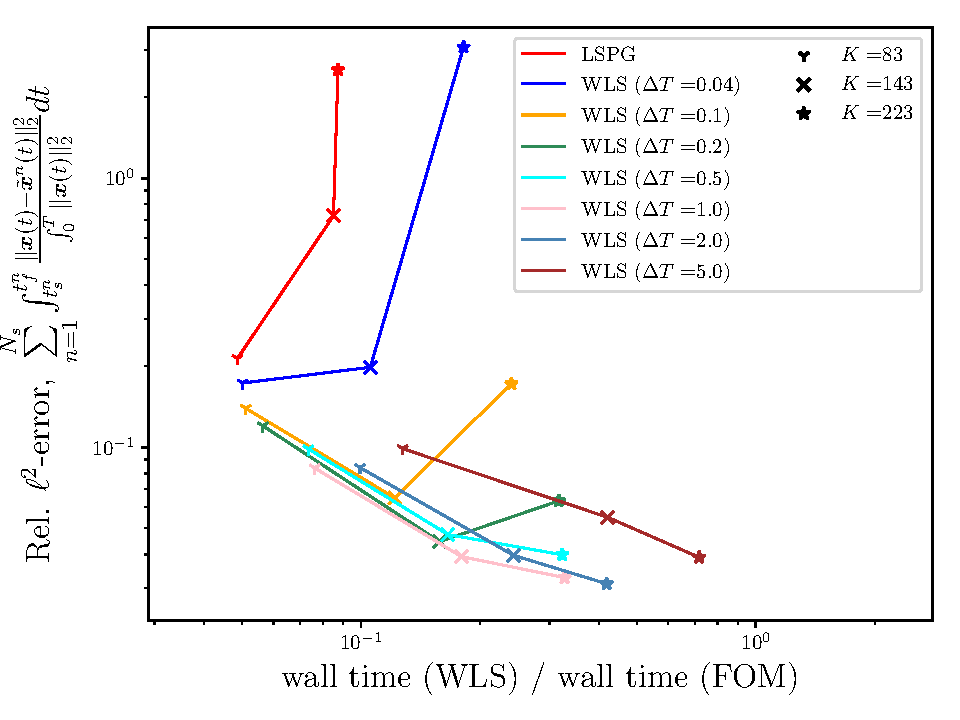
\includegraphics[trim={0cm 0cm 0cm 0cm},clip,width=1.0\linewidth]{figs/swe/swe_converge_error_pareto.pdf}
%\caption{Relative time-inegrated $\elltwo$-error.}
\end{subfigure}
\begin{subfigure}[t]{0.49\textwidth}
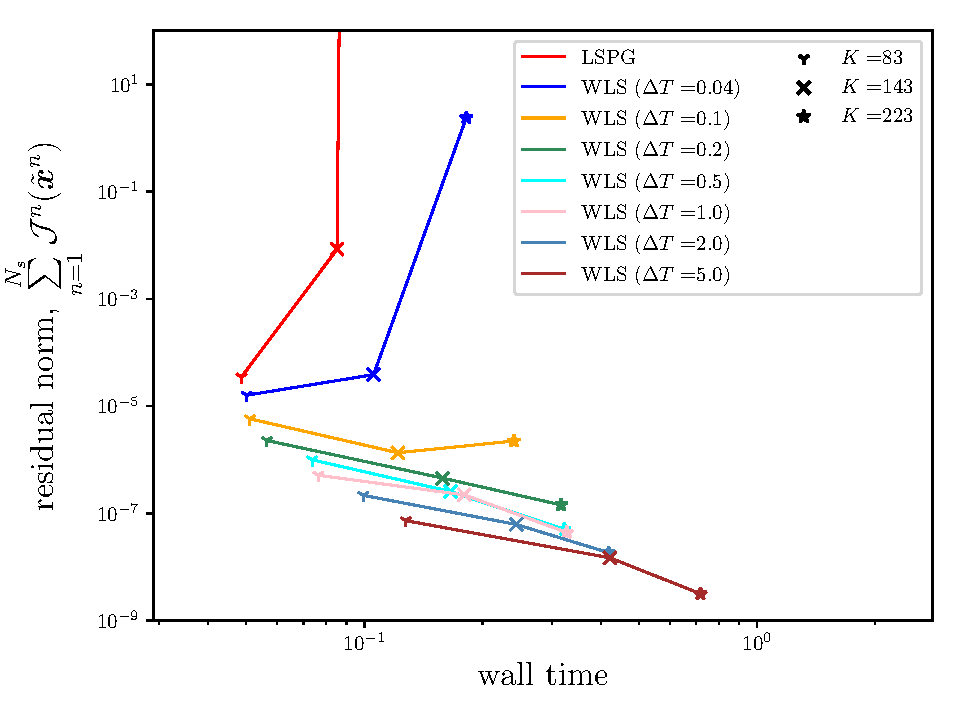
\includegraphics[trim={0cm 0cm 0cm 0cm},clip,width=1.0\linewidth]{figs/swe/swe_converge_resid_pareto.pdf}
%\caption{Time integrated residual norm.}
\end{subfigure}
%\begin{subfigure}[t]{0.85\textwidth}
\caption{Pareto fronts for the time-integrated $\elltwo$-error (left) and time-integrated residual (right) for LSPG and WLS ROMs.} 
\label{fig:rom_swe_pareto}
\end{center}
\end{figure}

